% !TeX spellcheck = fr_FR
\section{Développement du moteur et de l'interface}
	\begin{frame}
		\frametitle{Développement du moteur et de l'interface}
		\framesubtitle{Le moteur du jeu}
		\begin{figure}[h]
			\centering
			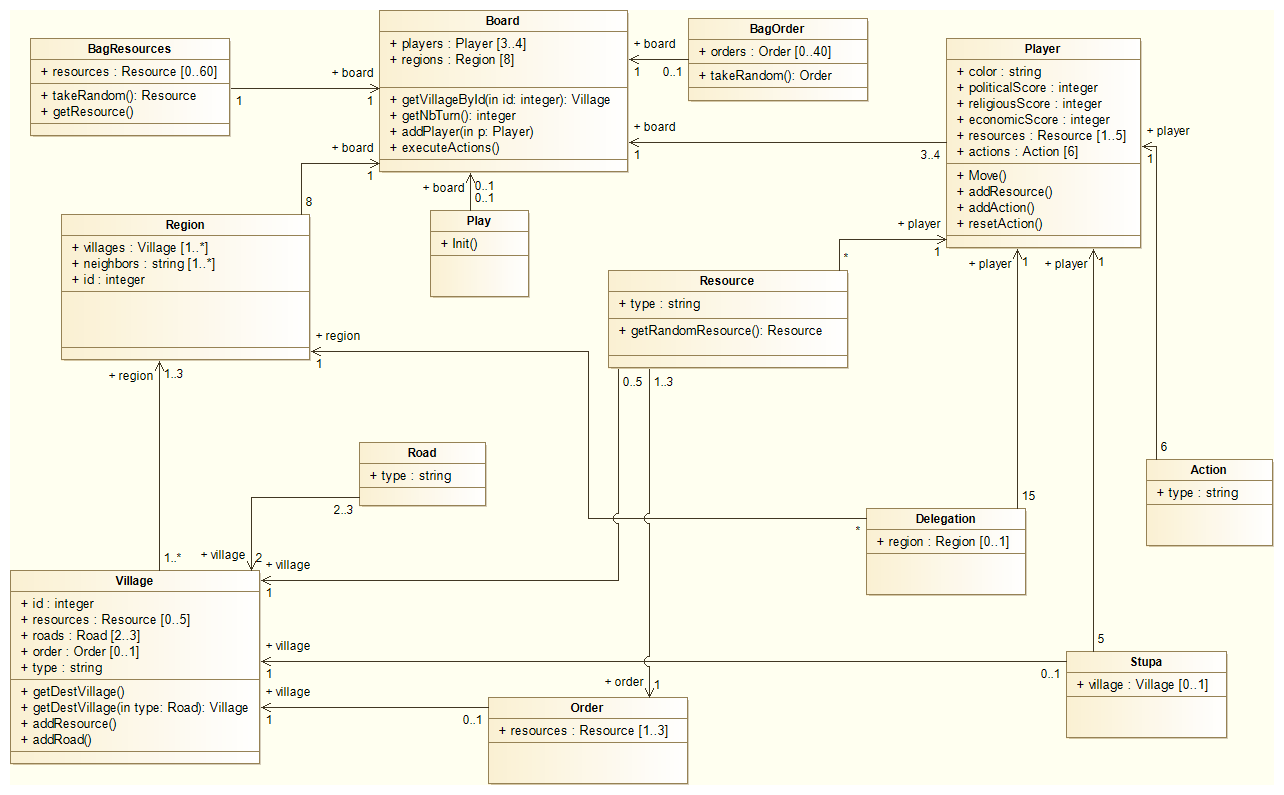
\includegraphics[width=0.8\linewidth]{images/UML_Himalaya_2}
			\caption{UML créé avant le développement}
			\label{fig:uml}
		\end{figure}
		
	\end{frame}

	\begin{frame}
		\frametitle{Développement du moteur et de l'interface}
		\framesubtitle{Le moteur du jeu}
		\begin{figure}[h]
			\centering
			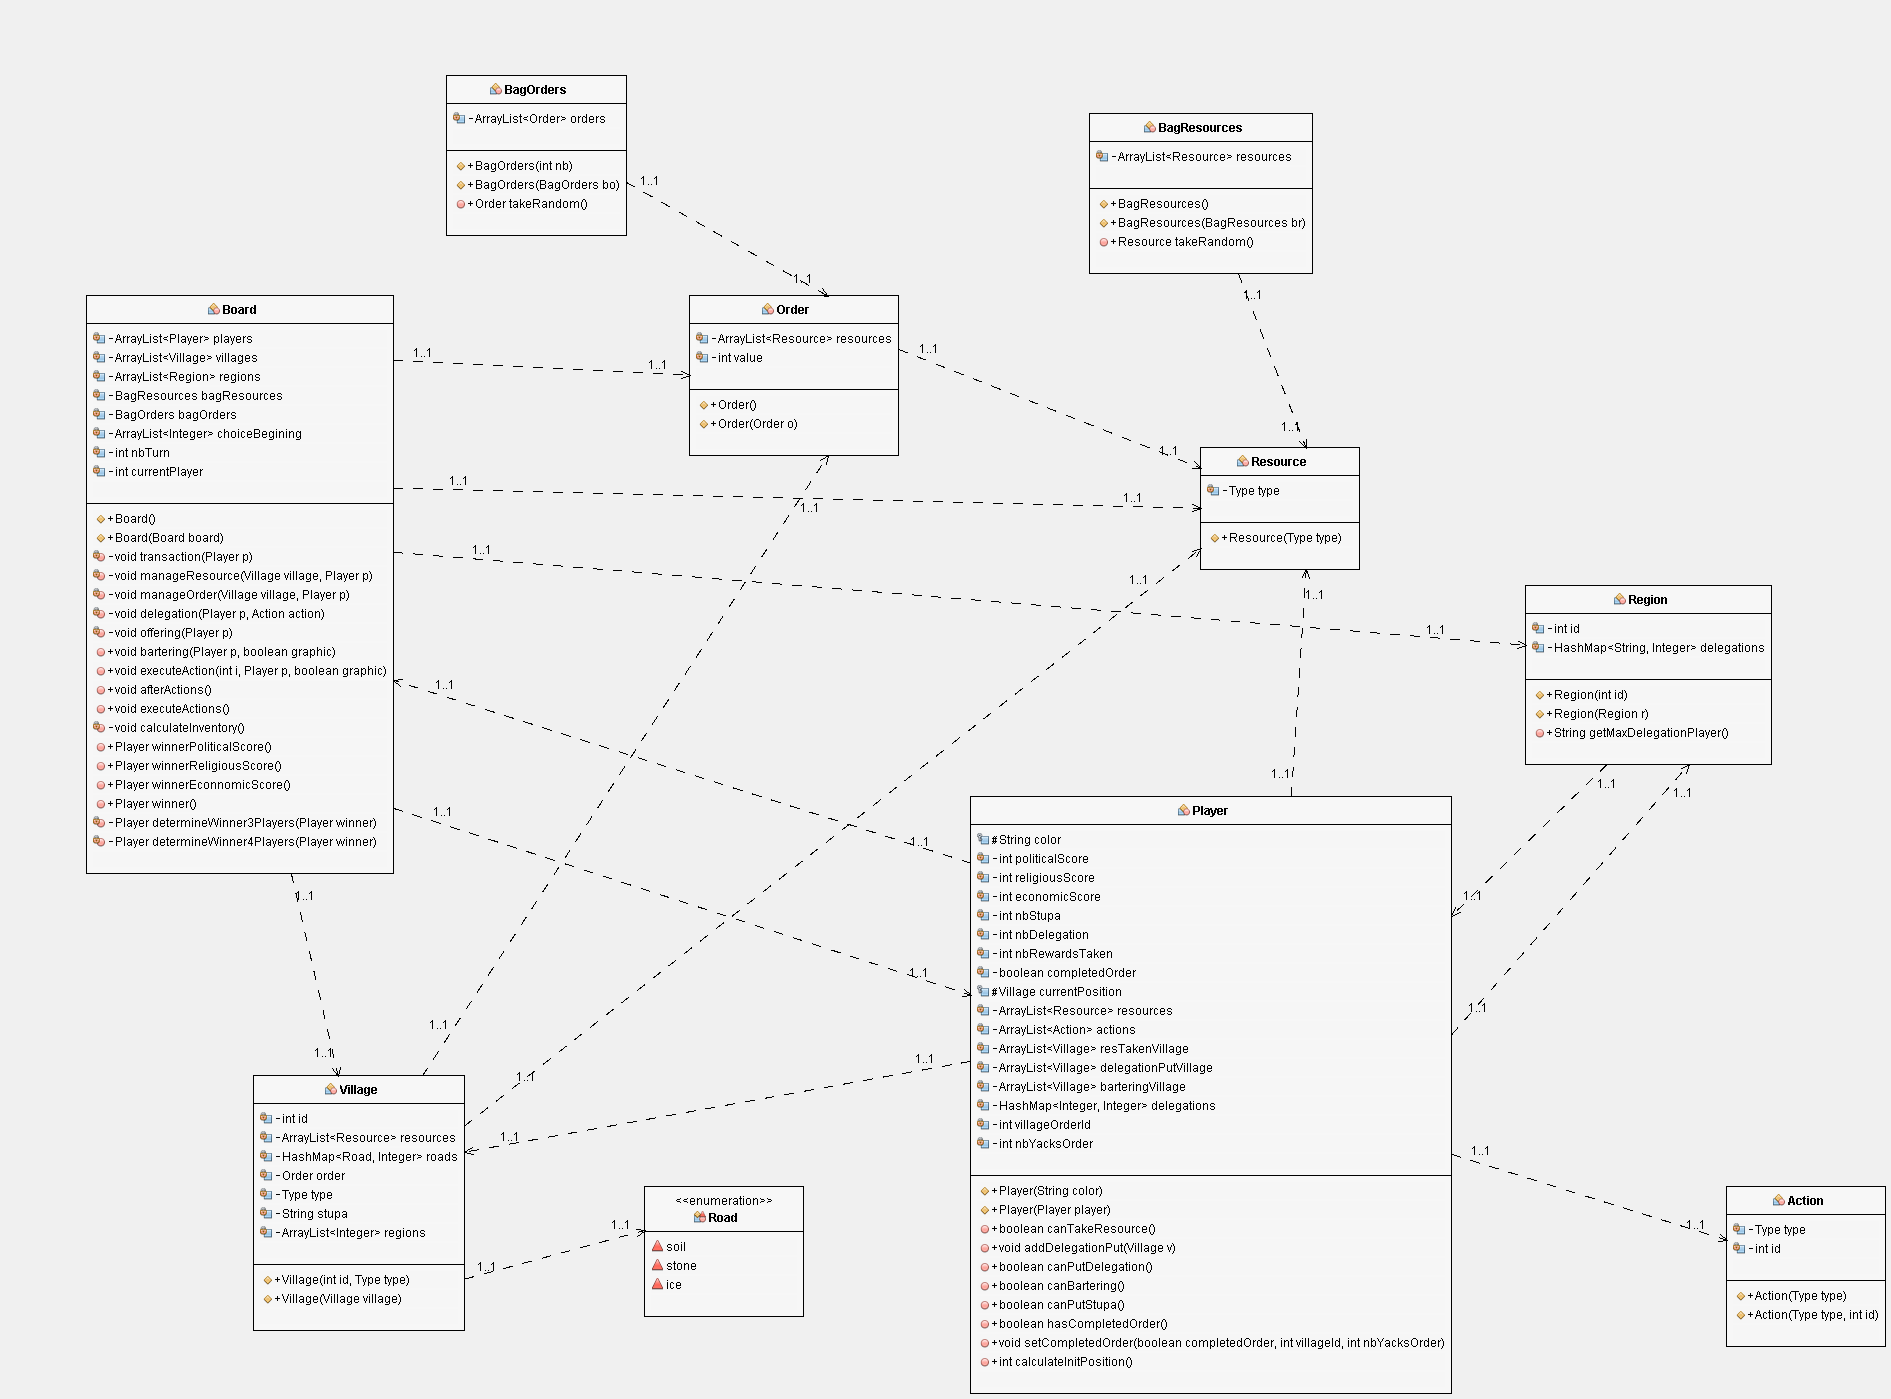
\includegraphics[width=0.8\linewidth]{images/UML_Himalaya_CORE_3}
			\caption{UML généré après le développement}
			\label{fig:uml}
		\end{figure}
	\end{frame}

	\begin{frame}
		\frametitle{Développement du moteur et de l'interface}
		\framesubtitle{Le moteur du jeu}
		\begin{block}{Le moteur}
			\begin{itemize}
				\item Utilisable pour version Graphique et Console
				\item Tests unitaires
				\item Classe Player avec classes fille IA
			\end{itemize}
		\end{block}	
	\end{frame}

	\begin{frame}
		\frametitle{Développement du moteur et de l'interface}
		\framesubtitle{L'interface graphique du jeu}
		\begin{block}{\fx}
			\begin{itemize}
				\item Pour chaque page : fichier \fxml et Controller 
				\item Création d'un "Framework" pour navigation entre les pages
				\item Utilisation du "Scene Builder" avec NetBeans
			\end{itemize}
		\end{block}	
	\end{frame}
	
	\begin{frame}
		\frametitle{Développement du moteur et de l'interface}
		\framesubtitle{L'interface graphique du jeu}
		\begin{figure}[h]
			\centering
			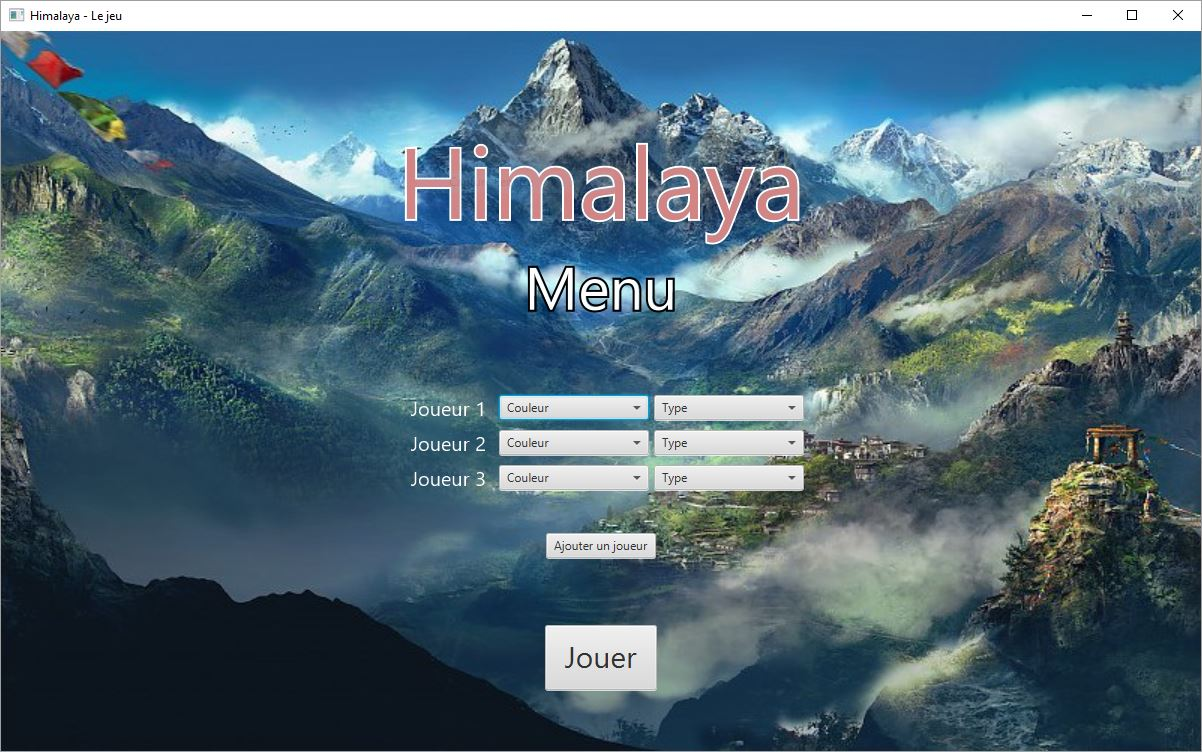
\includegraphics[width=0.8\linewidth]{images/menu}
			\caption{Menu du jeu}
			\label{fig:menu}
		\end{figure}
	\end{frame}
	
	\begin{frame}
		\frametitle{Développement du moteur et de l'interface}
		\framesubtitle{L'interface graphique du jeu}
		\begin{figure}
			\begin{subfigure}{0.5\textwidth}
				\centering
				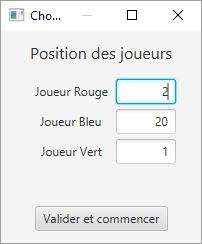
\includegraphics[width=0.4\linewidth]{images/position}
				\caption{Position Joueur}
				\label{fig:position}
			\end{subfigure}
			\begin{subfigure}{0.4\textwidth}
				\centering
				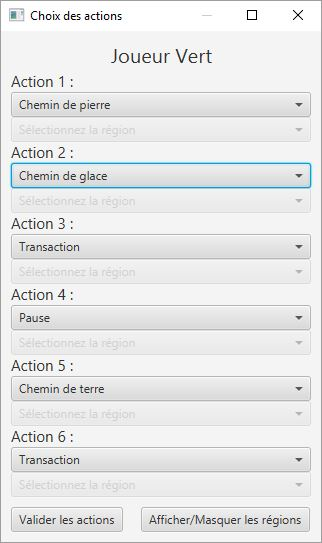
\includegraphics[width=0.5\linewidth]{images/actions}
				\caption{Fenêtre des actions}
				\label{fig:actions}
			\end{subfigure}
		\end{figure}
	\end{frame}

	\begin{frame}
		\frametitle{Développement du moteur et de l'interface}
		\framesubtitle{L'interface graphique du jeu}
		\begin{figure}[h]
			\centering
			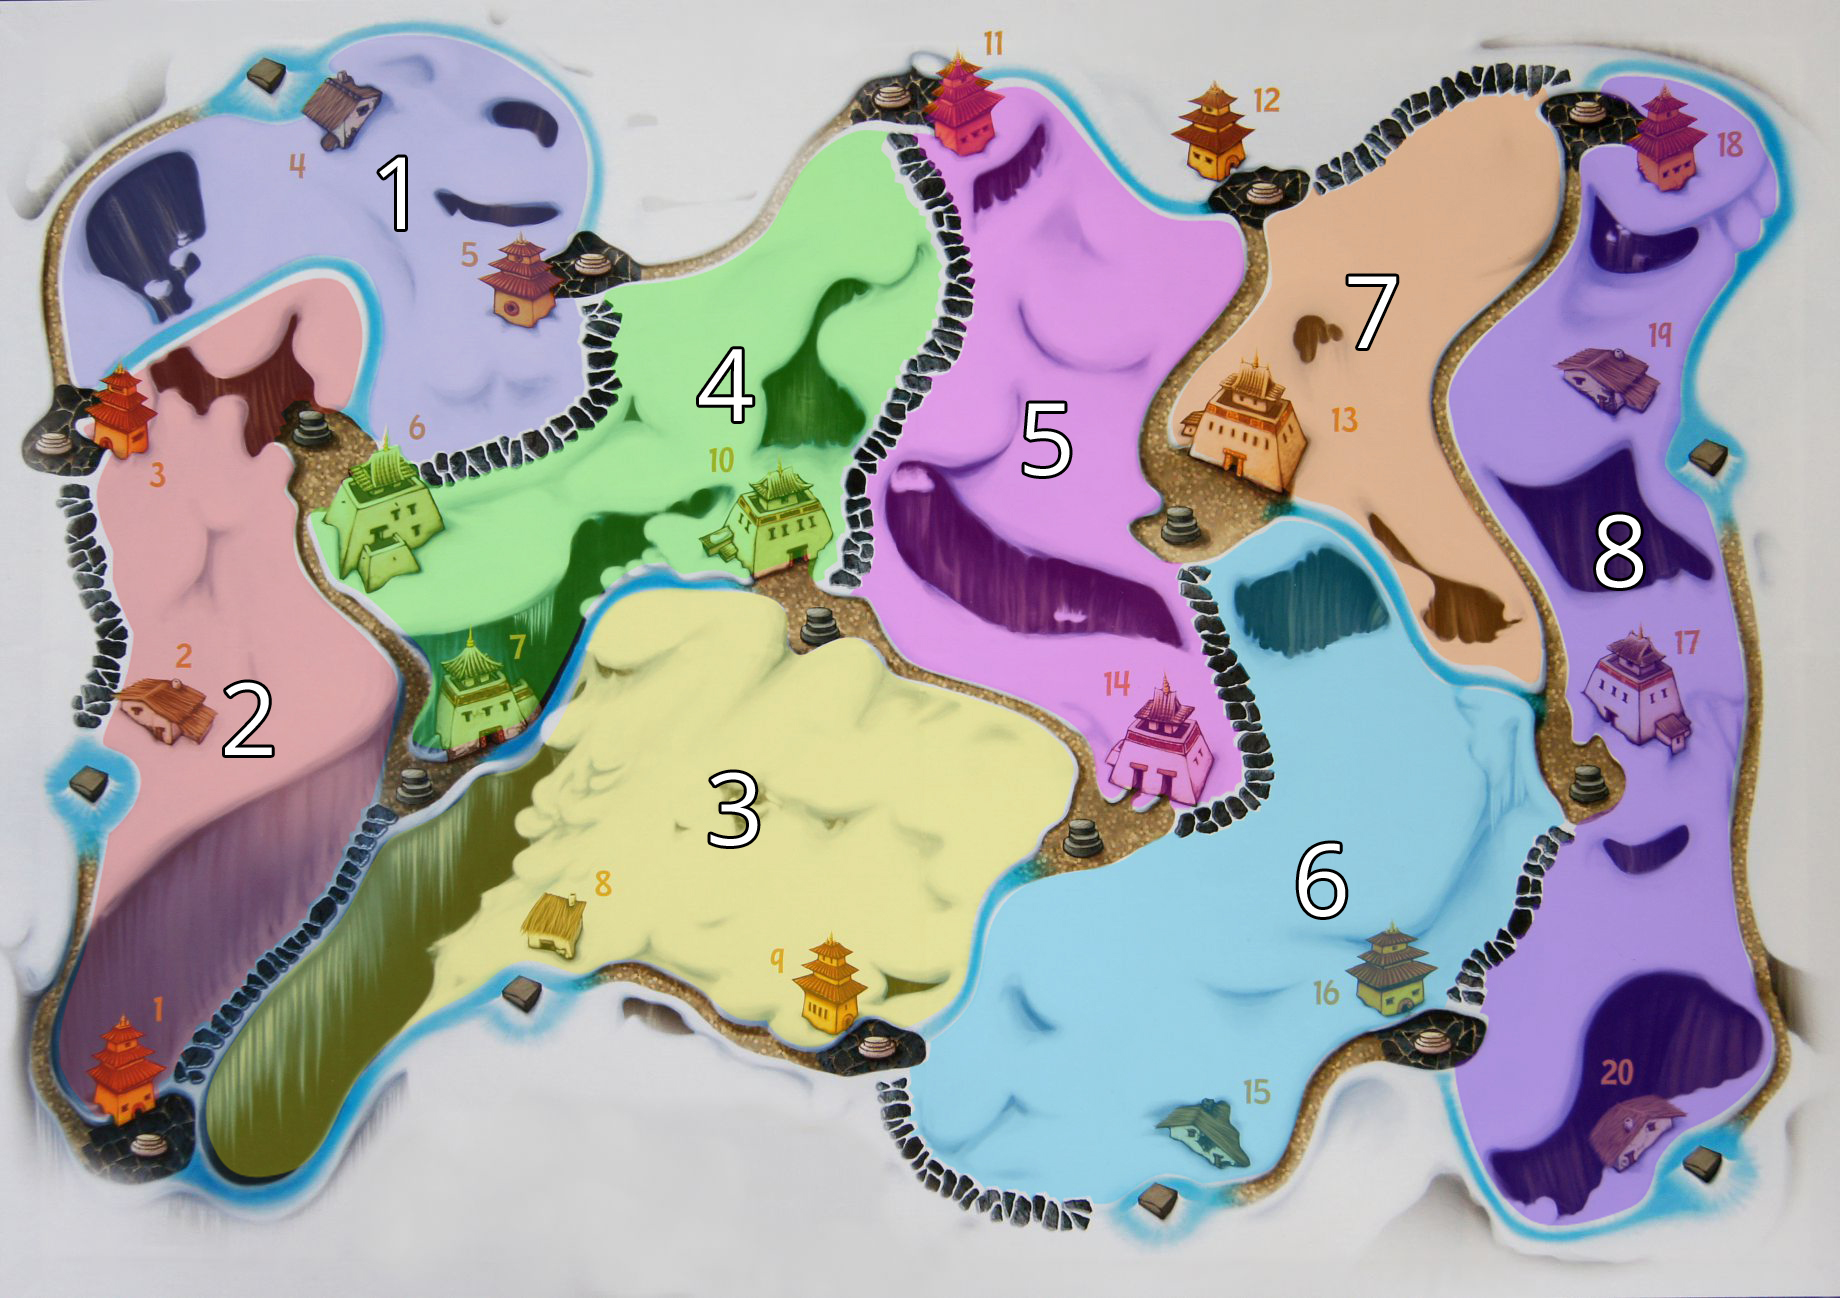
\includegraphics[width=0.8\linewidth]{images/board_regions}
			\caption{Régions sur le plateau}
			\label{fig:regions}
		\end{figure}
	\end{frame}

	\begin{frame}
		\frametitle{Développement du moteur et de l'interface}
		\framesubtitle{L'interface graphique du jeu}
		\begin{figure}[h]
			\centering
			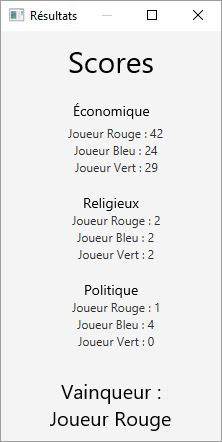
\includegraphics[width=0.25\linewidth]{images/resultats}
			\caption{Page de victoire}
			\label{fig:victoire}
		\end{figure}
	\end{frame}



	

